\documentclass[submit]{harvardml}

\course{CS181-S20}
\assignment{Assignment \#5}
\duedate{7:59pm EST, April 2, 2021}

\newcommand{\attr}[1]{\textsf{#1}}
\usepackage[OT1]{fontenc}
\usepackage[colorlinks,citecolor=blue,urlcolor=blue]{hyperref}
\usepackage[pdftex]{graphicx}
\usepackage{subfig}
\usepackage{framed}
\usepackage{fullpage}
\usepackage{amsmath}
\usepackage{amssymb}
\usepackage{color}
\usepackage{todonotes}
\usepackage{listings}
\usepackage{common}
\usepackage{bm}
\usepackage{enumitem}
\usepackage{tikz}
\usetikzlibrary{positioning,shapes,arrows}
\usepackage{xifthen}
\usepackage{soul}
\usepackage{float}


\usepackage[mmddyyyy,hhmmss]{datetime}

\definecolor{verbgray}{gray}{0.9}

\lstnewenvironment{csv}{
  \lstset{backgroundcolor=\color{verbgray},
  frame=single,
  framerule=0pt,
  basicstyle=\ttfamily,
  columns=fullflexible}}{}

\begin{document}


\begin{center}
{\Large Homework 5: EM with Mixtures, PCA, and Graphical Models}\\
\end{center}

This homework assignment will have you work with EM for mixtures, PCA,
and graphical models. We encourage you to read sections 9.4 and 8.2.5 of the course textbook.

Please type your solutions after the corresponding problems using this
\LaTeX\ template, and start each problem on a new page.

Please submit the \textbf{writeup PDF to the Gradescope assignment `HW5'}. Remember to assign pages for each question.

Please submit your \textbf{\LaTeX\ file and code files to the Gradescope assignment `HW5 - Supplemental'}. 


\begin{problem}[Expectation-Maximization for Categorical-Geometric Mixture Models, 25pts]

In this problem we will explore expectation-maximization for a
Categorical-Geometric Mixture model.

Specifically, we assume that there are a set of $K$ parameters $p_k
\in [0,1]$.  To generate each observation $n$, we first choose which
of those $K$ parameters we will use based on the (unknown) overall
mixing proportion over the components $\btheta \in [0,1]^K$,
where~${\sum_{k=1}^K \theta_k=1}$.  Let the (latent) $\boldz_n$ indicate
which of the $K$ components we use to generate observation $n$.  Next
we sample the observation $x_n$ from a geometric distribution
with parameter $p_{\boldz_n}$.  This process can be written as: 
\begin{eqnarray*}
 \boldz_n &\sim& \text{Categorical}(\btheta) \\
 x_n &\sim& \text{Geometric}(p_{\boldz_n} )
\end{eqnarray*}
We encode observation $n$'s latent
component-assignment ${\boldz_n \in
  \{0,1\}^K}$ as a one-hot vector. Element indicator variables $z_{n k}$ equal 1 if $\boldz_n$ was generated using component $k$.

A geometric distribution corresponds to the number of trials
needed to get to the first success. If success occurs with probability
$p$, its PMF is given by $p(x_n ; p_k) = (1 - p_k)^{x_n - 1} p_k$, where $x_n \in \{1, 2, ...\}$.

  \begin{enumerate}

  \item \textbf{Intractability of the Data Likelihood} We are
    generally interested in finding a set of parameters $p_k$ that
    maximize the data likelihood $\log
    p(\{x_n\}^N_{n=1}; \btheta, \{p_k\}^K_{k = 1})$.  Expand the data
    likelihood to include the necessary sums over observations
    $x_n$ and to marginalize out (via more sums) the latents
    $\boldz_n$.  Why is optimizing this likelihood directly
    intractable?  

\item \textbf{Complete-Data Log Likelihood} The complete data
  $D = \{(x_n, \boldz_n)\}_{n=1}^N$ includes latents $\boldz_n$. Write
  out the complete-data negative log likelihood. Apply the ``power
  trick''  and simplify your expression using indicator elements $z_{n
    k}$. \footnote{The ``power trick'' is used when terms in a PDF are raised to the power of indicator components of a one-hot vector.  For example, it allows us to rewrite $p(\boldz_n ;  \btheta) = \prod_k \theta_k^{z_{nk}}$.}

\[\mcL(\btheta, \{p_k\}^K_{k=1}) =  -\ln p(D; \btheta, \{p_k\}^K_{k=1}).\]

Note that optimizing
  this loss is now computationally tractable if we know $\boldz_n$.

\item \textbf{Expectation Step} Our next step is to introduce a
  mathematical expression for $\boldq_n$, the posterior over the
  hidden component variables~$\boldz_n$ conditioned on the observed data
  $x_n$ with fixed parameters.
That is:
  \begin{align*}
    \textbf{q}_n &= \begin{bmatrix}
      p(\boldz_n =\boldC_1| x_n; \btheta, \{ p_k \}^K_{k=1})
      \\
      \cdots
      \\
      \cdots
      \\
      p(\boldz_n =\boldC_K| x_n; \btheta, \{ p_k \}^K_{k=1})
    \end{bmatrix} 
  \end{align*}
  where $\boldC_k$ is a 1-hot encoded vector to represent component $k$.
  %
%
\begin{itemize}
\item  \textbf{Part 3.A } Write down and simplify the expression for
  $\boldq_n$.  Note that because the $\boldq_n$ represents the
  posterior over the hidden categorical variables $\boldz_n$, the
  components of vector $\boldq_n$ must sum to 1.
The main work is to find an expression for $p(\boldz_n|x_n; \btheta, \{p_k\}^K_{k=1})$  for any choice of $\boldz_n$; i.e., for any 1-hot encoded $\boldz_n$. With this, you can then construct the different components that make up the vector $\boldq_n$.
  

\item  \textbf{Part 3.B } Give a concrete  algorithm for calculating
  $\boldq_n$ for each example $x_n$, given parameters~$\btheta$ and~$\{ p_k\}^K_{k=1}$.

\end{itemize}


  (Continued on next page.)
\end{enumerate}

\end{problem}

\newpage


\begin{framed}
\noindent\textbf{Problem 1} (cont.)\\
\begin{enumerate}

  
\item[4.] \textbf{Maximization Step}
Using the~$\boldq_n$ estimates from the Expectation Step, derive an update for maximizing the expected complete data log likelihood in terms of~$\btheta$ and~$\{ p_k \}^K_{k=1}$.

\begin{itemize}
    \item \textbf{Part 4.A } Derive an expression for the expected complete-data log likelihood using $\boldq_n$.
    \item \textbf{Part 4.B } Find an expression for $\btheta$ that maximizes this expected complete-data log likelihood. You may find it helpful to use Lagrange multipliers in order to enforce the constraint $\sum \theta_k = 1$. Why does this optimal $\btheta$ make intuitive sense?
    \item \textbf{Part 4.C } Find an expression for the $\{p_k \}^K_{k = 1}$ that maximize the expected
      complete-data log likelihood.  Why does this optimal $\{p_k \}^K_{k = 1}$  make intuitive sense?
    \end{itemize}
    
\item[5.] Suppose that this had been a classification problem. That is,
  you were provided the ``true'' components $\boldz_n$ for each
  observation $x_n$,
  and you were going to perform the classification by
  inverting the provided generative model (i.e. now you're predicting $\boldz_n$ given $x_n$). Could you reuse any of
  your derivations above to estimate the parameters of the model?
  

\item[6.] Finally, implement your solution (see \texttt{T5\_P1.py} for starter code).  You are responsible for implementing the \texttt{expected\_loglikelihood}, \texttt{e\_step} and \texttt{m\_step} functions. Test it out with data given
  $10$ samples from $3$ components with $p_1 = .1$, $p_2=.5$, and
  $p_3=.9$.  How does it perform?  What if you increase the number of
  samples to $1000$ from each of the components?  What if you change
  $p_2=.2$?  Hypothesize reasons for the differences in performance
  when you make these changes. You may need to record five to ten trials (random restarts) in order to observe meaningful insights.
\end{enumerate}
  
\end{framed}  

\subsection*{Solution 1}

\begin{enumerate}
    \item \textbf{Expand the data likelihood to include the necessary sums over the observations $x_n$.}
    
    \begin{align*}
        p(x_n, \btheta, p_k) &= p(x_n | z_n = C_k, \theta) p(z_n = C_k) \\
        &= p(x_n | z_n = C_k) \btheta_k \\
        \log p(\{x_n\}^N_{n=1}; \btheta, \{p_k\}^K_{k = 1}) &= \log [\prod^n \sum^k p(x_n| z_n = C_k) \btheta_k]\\
        &=  \sum^n  \log [ \sum^k p(x_n| z_n = C_k) \btheta_k]
    \end{align*}
    
    This is intractable because there is a sum inside the log - this solution is not convex. Maximising over lambda and theta would have at least K unknowns. 
    
    \item \textbf{Complete-Data Log likelihood}\\
    Using our answer from 1.1:
    \begin{align*}
        \mcL(\btheta, \{p_k\}^K_{k=1}) &=  -\ln p(D; \btheta, \{p_k\}^K_{k=1}) \\
        -\ln p(D; \btheta, \{p_k\}^K_{k=1}) &= -\log \prod^n p(x_n| z_n = C_k) \btheta_k \\
        &= - \sum^n \sum^k \log [  ( p(x_n| z_n = C_k) \btheta_k)^{z_{nk}} ] \\
        \text{using log rules}\\
        &= - \sum^n \sum^k z_{nk} \log  ( p(x_n| z_n = C_k) \btheta_k)\\
    \end{align*}
    This now makes the computation tractable for a given set of $z_n$ values, we no longer have to worry about taking the log of a sum of numbers - we only need to sum a computed log of out equation.
    
    \item \textbf{Expectation Step:}
    \begin{enumerate}
        \item \textbf{Write down and simplify the expression for $q_n$}
        $q_n$ is the posterior over the hidden component variables. We can therefore find an expression for the $k_{th}$ value of each of the $q_n$.
        $$
            q_{nk} = p(z_n = C_k | x_n, \btheta, \{p_k\}^K_{k=1})
        $$
        Therefore we can write this as:
        \begin{align*}
            q_{nk} &= \frac{p(z_n = C_k | x_n, z, \theta)\btheta_k) }{\sum^K_{k=1} p(z_n = C_k | x_n, z, \theta)\btheta_k}\\
            &= \frac{(1 - p_k)^{x_n - 1} p_k\btheta_k) }{\sum^K_{k=1} (1 - p_k)^{x_n - 1} p_k\btheta_k}
        \end{align*}
        
        \item \textbf{Give a concrete algorithm for calculating $q_n$}\\
        To make an algorithm for calculating each $q_n$ we can use the following protocol:\\
        1. Compute the PMF and multiply it by the class probability ($\btheta_k$\\
        2. Normalize the vector to make the probabilities sum to 1\\
        
        \textbf{This can be written in python as:}
\begin{verbatim}
row = np.array([self.pmf(self.data[n], self.probs[k])*self.pis[k] for k in range(K)])
self.q[n] = row/np.sum(row)
\end{verbatim}
        
    \end{enumerate}
    \item \textbf{Maximisation step}
    \begin{enumerate}
        \item \textbf{Derive an expression for the expected complete-data log likelihood using $q_n$}\\
        Using our answer from problem 1.2, we know that the log likelihood is:
        $$\log p(\{x_n\}^N_{n=1}; \btheta, \{p_k\}^K_{k = 1}) = \sum^n \sum^k z_{nk} \log  ( p(x_n| z_n = C_k) \btheta_k)$$
        We can now simplify taking advantage of the linearity of expectation to simplify.\\
        \begin{align*}
            \mathbb{E} [ \log p(\{x_n\}^N_{n=1}; \btheta, \{p_k\}^K_{k = 1})] &= \mathbb{E} [\sum^n \sum^k z_{nk} \log  ( p(x_n| z_n = C_k) \btheta_k)]\\
            &= \sum^n \sum^k \mathbb{E} [z_{nk}  \log  ( p(x_n| z_n = C_k) \btheta_k)]\\
        \end{align*}
        
        We can split the logs and distribute the Expectations, we can also use 1.3 and substitute in our values of $q_nk$ for the predicted class (i.e. expected values) of each $z_nk$\\
        \begin{align*}
            &= \sum^n \sum^k \mathbb{E} [z_{nk}  \log  ( p(x_n| z_n = C_k))] + \mathbb{E} [z_{nk}  \log( \btheta_k)]\\
            &= \sum^n \sum^k \mathbb{E} [z_{nk}]  \log  ( p(x_n| z_n = C_k)) + \mathbb{E} [z_{nk}]  \log( \btheta_k)\\
            &= \sum^n \sum^k q_{nk}  \log  ( p(x_n| z_n = C_k)) + q_{nk}  \log( \btheta_k)\\
        \end{align*}
        
        \item \textbf{Derive an expression for $\btheta$ that maximises the log loss}
        Here we can take the derivative of our loss function with respect to $\theta$ using Lagrange multipliers.
        
        \begin{align*}
            \mcL(\btheta, \{p_k\}^K_{k=1}) &= \sum^n \sum^k q_{nk}  \log  ( p(x_n| z_n = C_k)) + q_{nk}  \log( \btheta_k) + \lambda (1 - \sum^k \btheta_k)\\
        \end{align*}
        
        First we can take the partial derivative with respect to $\theta_k$:
        
        \begin{align*}
            \frac{d(\mcL(\btheta))}{d(\btheta_k)} &= \sum^n \sum^k q_{nk} \frac{1}{\btheta_k} + \lambda(-\sum^k 1)\\
            &= \sum^n \sum^k \frac{q_{nk}}{\btheta_k} + \lambda(-\sum^k 1) = 0 \\
            \lambda &= \sum^n \frac{q_{n}}{\btheta_k}
        \end{align*}
        
        Likewise we can now take the partial derivative of the loss with respect to $\lambda$:
        
        \begin{align*}
            \frac{d(\mcL(\btheta))}{d(\lambda)} &= 1 - \sum^k \btheta_k\\
            \sum^k \btheta_k = 1
        \end{align*}
        
        Putting this together we can see:
        \begin{align*}
            \btheta_k = \frac{1}{N} \sum^n q_n\\
        \end{align*}
        This makes intuitive sense as we are finding the proportion of data points that exist for a given class - this is exactly what $\theta_k$ is representing, the probability of a given point existing in a given class.
        \item \textbf{Find an expression for the $p_k$ that maximises the expected the complete-data log likelihood.}
        First we can simplify and substitute in the PMF:
        \begin{align*}
            \mcL(\btheta, \{p_k\}^K_{k=1}) &= \sum^n \sum^k q_{nk}  \log  ( p(x_n| z_n = C_k)) + q_{nk}  \log( \btheta_k)\\
            &= \sum^n \sum^k q_{nk}  \log  ( (1 - p_k)^{x_n - 1} p_k ) + q_{nk}  \log( \btheta_k)\\
            &= \sum^n \sum^k q_{nk}  (x_n - 1)\log (1 - p_k) +\log(p_k) + q_{nk}  \log( \btheta_k)\\
        \end{align*}
        As before, we can take the derivative of our loss function with respect to $p_k$:
        \begin{align*}
            \frac{d(\mcL(\btheta))}{d(\btheta_k)} &= \sum^n \sum^k \frac{q_{nk}(x_n - 1)}{(1 - p_k)} +\frac{1}{p_k} = 0\\
            p_k &= \frac{q_{nk}}{q_{nk} x_n}
        \end{align*}
        This makes intuitive sense as we are finding the number of x values in a given class divided by the sum of the x values for that class - thereby finding the geometric distribution parameters.
    \end{enumerate}
    \item \textbf{Could you reuse any of your derivations above to estimate the parameters of the new model?}\\
    The derivations above can be reused, we now have the values of $z_n$ so we can predict the $\theta_k$ and $p_k$. 
    We essentially would only have to repeat the "M - Step" of the algorithm, every time we would be using a $q_n$ we can substitute in $z_n$:
    
    \begin{align*}
        p_k &= \frac{\sum^n z_{nk}}{\sum^n z_{nk} x_n}\\
        \theta_k &= \frac{1}{N} \sum^n z_{nk}\\
    \end{align*}
   \item \textbf{Implement the model in \textit{T5\_P1.py}, what are the results?}\\
   
   When given 10 samples from 3 components with $p_1 = 0.1$, $p_2 = 0.5$, $p_3 = 0.9$, the model performs as follows:\\
   \textbf{Accuracy}: $73.33\%$\\
   \textbf{Probabilities}: $[0.05400968, 0.51898827, 0.77010694]$\\
   
   When given 1000 samples from 3 components with $p_1 = 0.1$, $p_2 = 0.5$, $p_3 = 0.9$, the model performs as follows:\\
   \textbf{Accuracy}: $61.2\%$\\
   \textbf{Probabilities}: $[0.09302592, 0.22965224, 0.7672521]$\\
   
   Now when changing $p2$:\\
   When given 10 samples from 3 components with $p_1 = 0.1$, $p_2 = 0.2$, $p_3 = 0.9$, the model performs as follows:\\
   \textbf{Accuracy}: $56.66\%$\\
   \textbf{Probabilities}: $[0.1869832,  0.25130479, 0.72401298]$\\
   
   When given 1000 samples from 3 components with $p_1 = 0.1$, $p_2 = 0.2$, $p_3 = 0.9$, the model performs as follows:\\
   \textbf{Accuracy}: $60.3\%$\\
   \textbf{Probabilities}: $[0.11210157, 0.31694061, 0.95508395]$\\
   
   
   Overall, the model performs very quickly over 10 samples and comparatively slower over 1000 samples, this is due to the log likelihoods taking longer to converge. The difference in performance between a $p_2=0.5$ vs a $p_2=0.2$ is due to there being a lower chance of seeing an outcome with a lower probability - (a longer time for a Heads or a success in our geometric distribution) - while the probabilities will converge with more trials, it is hard to see convergence for low probabilities over small trials as there are simply not enough results. The restarts allow us to see a trial where we have good and bad luck when approximating these probabilities.
\end{enumerate}

\newpage

\begin{problem}[PCA, 15 pts]

For this problem you will implement PCA from scratch.  Using
\texttt{numpy} to call SVDs is fine, but don't use a third-party
machine learning implementation like \texttt{scikit-learn}.

We return to the MNIST data set from T4. You have been given
representations of 6000 MNIST images, each of which are $28\times28$
greyscale handwritten digits. Your job is to apply PCA on MNIST, and
discuss what kind of structure is found.

The given code in \texttt{T5\_P2.py} loads the images into your environment.  File \texttt{T5\_P2\_Autograder.py} contains a test case to check your cumulative proportion of variance.

\begin{enumerate}

\item Compute the PCA. Plot the eigenvalues corresponding to the most significant 500
  components in order from most significant to least. Make another plot that describes the cumulative proportion of variance explained by the first $k$ most significant components for values of $k$ from 1 through 500.
  How much variance is explained by the first 500 components?  Describe
  how the cumulative proportion of variance explained changes with $k$.

\item Plot the mean image of the dataset and plot an image corresponding to each of the
  first 10 principle components.  How do the principle component images compare to the
  cluster centers from K-means? Discuss any similarities and
  differences.  Include all 11 plots in your PDF submission.

\item Compute the reconstruction error on the data set using the mean
  image of the dataset. Then compute the reconstruction error using the first 10 principal components. How do these
  errors compare to the final objective loss achieved by using K-means on the dataset? Discuss any similarities and
  differences.

\end{enumerate}


\textit{Include your plots in your PDF. There may be several plots for this problem, so feel free
to take up multiple pages.}
\end{problem}

\newpage
\subsection*{Solution 2:}
\begin{enumerate}
    \item
    \begin{enumerate}
        \item 
        \textbf{Plot the Eigenvalues corresponding to the most significant 500 components in order from significant to least.}
        \begin{figure}[H]
            \includegraphics[width=8cm]{hw5/plots/2_1a.png}
            \centering
        \end{figure}
        
        \item \textbf{Plot the the cumulative proportion of variance explained by the first k significant components.}
        \begin{figure}[H]
            \includegraphics[width=8cm]{hw5/plots/2_1b.png}
            \centering
        \end{figure}
        \item \textbf{How much variance is explained by the first 500 components, describe the relationship between variance and k?}\\
        Looking at the graph, we can see that the relationship between the number of components and the variance in the model is logarithmic, with the graph approaching 1 as we near 500 principal components. The final value (i.e. the 500th) of the retained variance is $0.9999999999999993$ - practically all the variance. With only 100 principal components we are already explaining 90\% of the variation in the data. 
    \end{enumerate}
    
    \item 
    \begin{enumerate}
        \item \textbf{Plot the mean image of the dataset.}
        \begin{figure}[H]
            \includegraphics[width=8cm]{hw5/plots/2_2a.png}
            \centering
        \end{figure}
        \item \textbf{Plot an image corresponding to the first 10 principal components.}
        \begin{figure}[H]
            \includegraphics[width=18cm]{hw5/plots/2_2b.png}
            \centering
        \end{figure}
        \item \textbf{How do the principle component images compare to the k-means cluster center images?}\\
        These images look different to the K-means images in the sense that they are not classifying the types of digits - in K-means the cluster centers largely looked like an average value of the elements of a given cluster so in the case of a cluster of the digit $8$ the result would be a blurry $8$. Instead, these principal components there are sharper corners and unique features. These unique features can be interpreted as the locations of differentiation between the classes, looking at principal component 8, you can see the highly angular features of a 4 or a 7 and a lack of the curves of a 0 or an 8.
    \end{enumerate}
    
    \item 
    \begin{enumerate}
        \item \textbf{Compute the reconstruction error on the data set using the mean image.}\\
        The reconstruction error on the data set using the mean image is $5748048.794500034$.
        \item \textbf{Compute the reconstruction error on the first 10 components}\\
        The reconstruction error on the data set using the first 10 principal components is $1731315.3279392119$. Each data point was projected onto the 10 principal components and then projected back into the D dimensions.
        \item \textbf{How do these errors compare the final objective loss achieved by K-means?}\\
        The final objective loss by k-means are higher than the losses found here, we can see that as in the case with K-means, the more clusters and components we use, the lower the loss will be. It is intuitive that PCA will select 10 components that have a lower overall objective loss than K-mean as they are analytically found to describe the most amount of variance in the data - K-means has a degree of randomness determining the starting position of the cluster so it is likely that they will not find the optimal components. 
    \end{enumerate}
    
\end{enumerate}

\newpage

\begin{problem}[Bayesian Networks, 10 pts]

  \noindent In this problem we explore the conditional independence
  properties of a Bayesian Network.  Consider the following Bayesian
  network representing a fictitious person's activities. Each random
  variable is binary (true/false).

\begin{center}
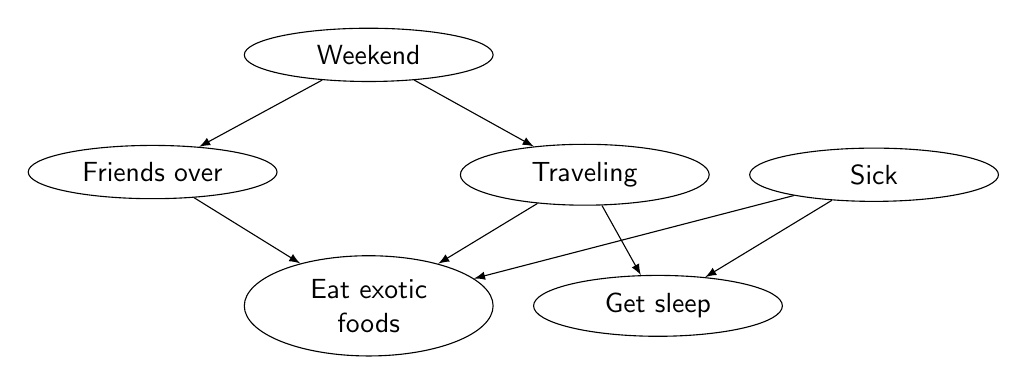
\begin{tikzpicture}[
  node distance=1cm and .5cm,
  bn/.style={draw,ellipse,text width=2cm,align=center}
    ]
    \node[bn] (w) {\attr{Weekend}};
    \node[bn,below right=of w] (t) {\attr{Traveling}};
    \node[bn,right=of t] (s) {\attr{Sick}};
    \node[bn,below left=of w] (f) {\attr{Friends over}};
    \node[bn,below right=of f] (eef) {\attr{Eat exotic foods}};
    \node[bn,right=of eef] (gs) {\attr{Get sleep}};
    \path (w) edge[-latex] (t)
    (w) edge[-latex] (f)
    (f) edge[-latex] (eef)
    (t) edge[-latex] (eef)
    (t) edge[-latex] (gs)
    (s) edge[-latex] (gs)
    (s) edge[-latex] (eef);
    \end{tikzpicture}
\end{center}

The random variables are:

\begin{itemize}
\item \attr{Weekend}: Is it the weekend?
\item \attr{Friends over}: Does the person have friends over?
\item \attr{Traveling}: Is the person traveling?
\item \attr{Sick}: Is the person sick?
\item \attr{Eat exotic foods}: Is the person eating exotic foods?
\item \attr{Get Sleep}: Is the person getting sleep?
\end{itemize}

\medskip

For the following questions, $A \perp B$ means that events A and B are
independent and $A \perp B | C$ means that events A and B are independent
conditioned on C.

\textbf{Use the concept of d-separation} to answer the
questions and show your work (i.e., state what the blocking path(s) is/are and what nodes block the path; or explain why each path is not blocked).

\textit{Example Question:} Is $\attr{Friends over} \perp \attr{Traveling}$? If NO, give intuition for why.

\textit{Example Answer:} NO. The path from Friends over -- Weekend -- Traveling is not blocked following the d-separation rules. Thus, the two are not independent. Intuitively, this makes sense as if say we knew that the person was traveling, it would make it more likely to be the weekend. This would then make it more likely for the person to have friends over.

\textbf{Actual Questions:}

\begin{enumerate}
\item Is $\attr{Sick} \perp \attr{Weekend}$?
  If NO, give intuition for why.


\item Is $\attr{Sick} \perp \attr{Friends over}\given \attr{Eat exotic
  foods}$? If NO, give intuition for why.


\item Is $\attr{Friends over} \perp \attr{Get Sleep}$? If NO, give
  intuition for why.

\item Is $\attr{Friends over} \perp \attr{Get Sleep} \given
  \attr{Traveling}$? If NO, give intuition for why.

\item Suppose the person stops traveling in ways that affect their
  sleep patterns (as various famous people have done).  Travel still
  affects whether they eat exotic foods.  Draw the modified network. (Feel free to reference the handout file for the commands for displaying the new network in \LaTeX).

\item For this modified network, is $\attr{Friends over} \perp
  \attr{Get Sleep}$? If NO, give an intuition why.  If YES,
  describe what observations (if any) would cause them to no longer be
  independent.

\end{enumerate}
\end{problem}


\section*{Solution 3}

\begin{enumerate}
    \item Yes. "Sick" and "weekend" are independent. Using D-separation rules, we can see that paths of sick and weekend are blocked. This makes sense as the day of the week would not affect if a person is sick.
    \item No. "Sick" is not independent of "Friends over" given "Eat exotic foods". We can rewrite this as $\text{Sick} \rightarrow \text{Eat exotic foods} \leftarrow \text{Friends over}$ and see that it is on our network and not blocked as "Eat exotic foods" is observed. This makes sense as it is likely that if a person has friends over given that the ate exotic foods, it is likely that they are not sick.
    \item No. "Friends over" is not independent of "Get sleep", there is a path through travelling and weekend. Intuitevly this makes sense as a person with friends over is less likely to get sleep. 
    \item Yes. "Friends over" is independent of "Get sleep" when "Travelling" is observed. This is because observation of travelling blocks the path. Therefore, there is no path between "weekend" and "get sleep".
    \item The new network will remove the path between "Travelling" and "Get sleep":
    \begin{center}
    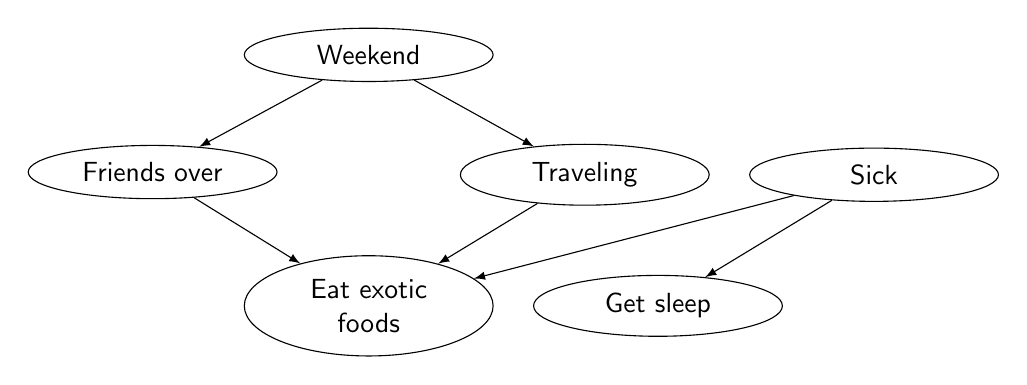
\begin{tikzpicture}[
      node distance=1cm and .5cm,
      bn/.style={draw,ellipse,text width=2cm,align=center}
        ]
        \node[bn] (w) {\attr{Weekend}};
        \node[bn,below right=of w] (t) {\attr{Traveling}};
        \node[bn,right=of t] (s) {\attr{Sick}};
        \node[bn,below left=of w] (f) {\attr{Friends over}};
        \node[bn,below right=of f] (eef) {\attr{Eat exotic foods}};
        \node[bn,right=of eef] (gs) {\attr{Get sleep}};
        \path (w) edge[-latex] (t)
        (w) edge[-latex] (f)
        (f) edge[-latex] (eef)
        (t) edge[-latex] (eef)
        % (t) edge[-latex] (gs)
        (s) edge[-latex] (gs)
        (s) edge[-latex] (eef);
        \end{tikzpicture}
    \end{center}
    
    \item Yes. "Friends over" is now independent of "Get Sleep". However, the independence would be broken if "Eat exotic foods" is observed. This intuitively makes sense, because given information about "eat exotic foods", we would change the likelihood of "Sick" and therefore effect the likelihood of "get sleep" therefore showing no independence. 
\end{enumerate}


\newpage
%%%%%%%%%%%%%%%%%%%%%%%%%%%%%%%%%%%%%%%%%%%%%
% Name and Calibration
%%%%%%%%%%%%%%%%%%%%%%%%%%%%%%%%%%%%%%%%%%%%%
\subsection*{Name}
Phil Labrum
\subsection*{Collaborators and Resources}
Natalie Margulies
Thomas Maldonado
Daniel Rodrigues

\subsection*{Calibration}
25 hours.

\end{document}
